\chapter{Radio neutrino detection}
\label{chap:RND}
In this chapter I'll explain how astrophysical neutrinos get detected in the
context of the Radio Neutrino Observatory in Greenland, or RNO-G.

Neutrinos are omnipresent in nature but as they interact very weakly we'll need
a big detector to detect reasonable amounts in finite timespans.  
To this end we can make use of a detector volume nature has
built for us: the Greenland icecap.  Even though various detector media
have been used, like water\cite{SuperKamio}, heavy water\cite{SNO:1999crp} and
even the moon\cite{numoon}, ice has been chosen as it has a few properties which makes it easy to
work with, of which some are listed below:
\begin{itemize}
  \item Ice is mostly see-through for electromagnetic radiation in the radio-frequency range
  \item The Greenland icecap is a really big continuous volume with little to no background from human activity
  \item As it's really cold within the ice, the detectors don't have to be made water-tight (contrary
	  to in-water detectors)
  \item As ice is a solid the detectors are logistically easy to deploy
\end{itemize}

To detect a neutrino it has to generate some kind of signal. As will be
explained, neutrinos can interact with hadronic matter to produce charged
particles. For cubic-kilometer type in-ice detectors these charged particles can then
be detected through the Cherenkov effect in the visible spectrum or
through the Askaryan effect in the radio frequency range.
For RNO-G the Askaryan effect will be leveraged.

\section{Neutrino interactions in ice}
\label{sec:NIII}
As neutrinos propagate through ice they can interact weakly with the nuclei .
The main mechanisms of interaction is via charged- and neutral current exchange
(see section \ref{sec:WeakInt}) with the quarks\cite{NuRadioMc} as is also
depicted in figure
\ref{fig:NeutrinoNucleusInteraction}.
\begin{figure}[h!]
	\begin{minipage}{\textwidth}
		\begin{minipage}{0.49\textwidth}
			\centering
			\begin{tikzpicture}
				\begin{feynman}
					\vertex (a0) {quark};
					\vertex[above=0.5cm of a0] (a1) {quark};
					\vertex[above=0.5cm of a1] (a2) {quark};
					\vertex[right=2cm of a0] (b0) {quark};
					\vertex[right=2cm of a1] (b1) {quark};
					\vertex[right=2cm of a2] (b2) {quark};
					\vertex[right=1.0cm of a2] (am);
					\vertex[above=1cm of am] (c0);
					\vertex[above=1cm of c0] (c1);
					\vertex[above=1cm of c1] (cm);
					\vertex[left=1cm of cm] (a3) {$\nu_l$};
					\vertex[right=1cm of cm] (b3) {$l$};
					\diagram* {
						{[edges=fermion]
							(a0) -- (b0)
						},
						{[edges=fermion]
							(a1) -- (b1)
						},
						{[edges=fermion]
							(a2) -- (c0) -- (b2)
						},
						{[edges=fermion]
							(a3) -- (c1) -- (b3)
						},
						{[edges=boson, edge label=W]
							(c0) -- (c1)
						},
					};
				\end{feynman}
			\end{tikzpicture}
		\end{minipage}
		\begin{minipage}{0.49\textwidth}
			\centering
			\begin{tikzpicture}
				\begin{feynman}
					\vertex (a0) {quark};
					\vertex[above=0.5cm of a0] (a1) {quark};
					\vertex[above=0.5cm of a1] (a2) {quark};
					\vertex[right=2cm of a0] (b0) {quark};
					\vertex[right=2cm of a1] (b1) {quark};
					\vertex[right=2cm of a2] (b2) {quark};
					\vertex[right=1.0cm of a2] (am);
					\vertex[above=1cm of am] (c0);
					\vertex[above=1cm of c0] (c1);
					\vertex[above=1cm of c1] (cm);
					\vertex[left=1cm of cm] (a3) {$\nu$};
					\vertex[right=1cm of cm] (b3) {$\nu$};
					\diagram* {
						{[edges=fermion]
							(a0) -- (b0)
						},
						{[edges=fermion]
							(a1) -- (b1)
						},
						{[edges=fermion]
							(a2) -- (c0) -- (b2)
						},
						{[edges=fermion]
							(a3) -- (c1) -- (b3)
						},
						{[edges=boson, edge label=Z]
							(c0) -- (c1)
						},
					};
				\end{feynman}
			\end{tikzpicture}
		\end{minipage}
	\end{minipage}
	\caption{Most prominent ways of neutrino-nucleus interaction}
	\label{fig:NeutrinoNucleusInteraction}
\end{figure}

The produced leptons in the W boson mediated interaction are either electrons,
resulting in an electromagnetic shower, muons which typically live
too long and thus escape the detector volume before they can deposit all of their 
energy in the ice\cite{PhdthesisWeling} or tauons which will decay via
\begin{equation}
	\tau^- \rightarrow e^- + \bar{\nu}_e + \nu_\tau
\end{equation}
or, less ideally
\begin{equation}
	\tau^- \rightarrow \mu^- + \bar{\nu}_\mu + \nu_\tau
\end{equation}
In both the charged and neutral current interaction, the resulting nucleus
will result in an hadronic shower. For the neutral current interaction
the fraction of the neutrino energy that gets transferred to
the nucleon is described by the inelasticity $y$ and is heavily shifted towards
small values of $y$\cite{elasticity_y}. This causes a big, irreducible
uncertainty when trying to estimate the original neutrino energy from these
kinds of events.  With the charged current interaction (mediated by the $W^\pm$
bosons) this isn't a problem however as the full neutrino energy ends up in the
resulting cascades.
\section{Askaryan effect}
\label{sec:Askaryan}
A particle shower in ice formed through the interactions described in section
\ref{sec:NIII} can emit strong radio signals if two conditions are met:
\begin{itemize}
	\item There is separation of positive and negative charges in the shower front 
	\item The signals produced over the length of the shower profile overlap coherently.
\end{itemize}
The \textit{Askaryan} \cite{Askaryan} effect, which is responsible for the
production of Askaryan radiation describes the effect at radio frequencies
which abides by both of these conditions.  In general it's a quite involved
effect but we'll give a crude overview. After neutrinos interact in the ice
they produce a cascade of secondary charged particles containing a net negative
charge anisotropy\cite{Connolly_2017}.  This charge imbalance is a result of
medium electrons either Compton scattering into the advancing shower or
annihilating with shower positrons.  This moving charge anisotropy is
propagating faster than the speed of light in the dielectric medium, creating
Cherenkov radiation.  

Cherenkov radiation can be considered the electromagnetic equivalent of a sonic boom. 
A sonic boom happens when an object goes faster than the speed of sound in the
medium; In the same way a particle emits Cherenkov radiation if it propagates faster than 
the speed of light in the medium.  Choosing the particle trajectory to lie along the z
axis an approximate equation can be found\cite{jackson1998classical} for
$\frac{\text{d}^2 \mathscr{J}}{\text{d}\omega \text{d}\Omega}$, which is the energy
radiated per elementary unit solid angle and per elementary unit frequency
interval:
\begin{equation}
	\frac{\text{d}^2 \mathscr{J}(\omega)}{\text{d} \omega \text{d} \Omega} = \frac{q^2}{4\pi}\sqrt{\frac{\mu}{\epsilon}}\beta^2\omega^2\delta^2[\omega(1-\beta \mathbf{e}_r\cdot\mathbf{e}_z)]|\mathbf{e}_r\times\mathbf{e}_z|^2 \label{equation: 4.128 in elektromagnetisme}
\end{equation}
Now we can re-write this equation in spherical coordinates, which gives $1-\beta \mathbf{e}_r\cdot\mathbf{e}_z = 1-\beta\cos(\theta_c)$ in the delta function. We thus only expect radiation if
\begin{equation}
\cos(\theta_c) = \frac{1}{\beta} = \frac{c'}{u} = \frac{c}{n}\cdot\frac{1}{u}
\end{equation}
With u the local speed of light in the medium and n the index of refraction, an optical
property of a medium which we'll later on thoroughly discuss.
If $u>\frac{c}{n}$, Cherenkov radiation will
be emitted along a cone surface with half angle $\frac{\pi}{2}-\theta_c$ as
illustrated in figure \ref{figure: Cherenkov illustratie}. Integrating equation
\ref{equation: 4.128 in elektromagnetisme} over the solid angle and formally
dividing by the time interval we get:
\begin{equation}
	\frac{\text{d}^2\mathscr{J}}{\text{d}\omega \text{d}t} = \frac{q^2}{4\pi}\sqrt{\frac{\mu}{\epsilon}}\beta\omega\left(1-\frac{1}{\beta^2}\right)	
\end{equation}
We see that the energy is proportional to $\omega$, so we expect that most
radiation will be emitted "in blue" with a cut-off frequency above which the
equation $\cos\theta = 1/(n\beta)$ can no longer be satisfied. This "in blue"
characteristic is responsible for the blue glow seen in nuclear reactors as
seen in figure \ref{figure: Cherenkov reactor} .  For ice the index of
refraction is roughly 1.78 in deep ice\cite{Bogorodsky1985}, so we expect an ultra-relativistic
particle to produce the most radiation at around 56° opening as 
\begin{equation}
	\cos(\theta_c) \approx \frac{1}{n} \implies \cos^{-1}\left(\frac{1}{1.78}\right)\approx 56\text{°}
\end{equation}
\begin{figure}
\centering
\begin{minipage}{0.45\textwidth}
	\centering
	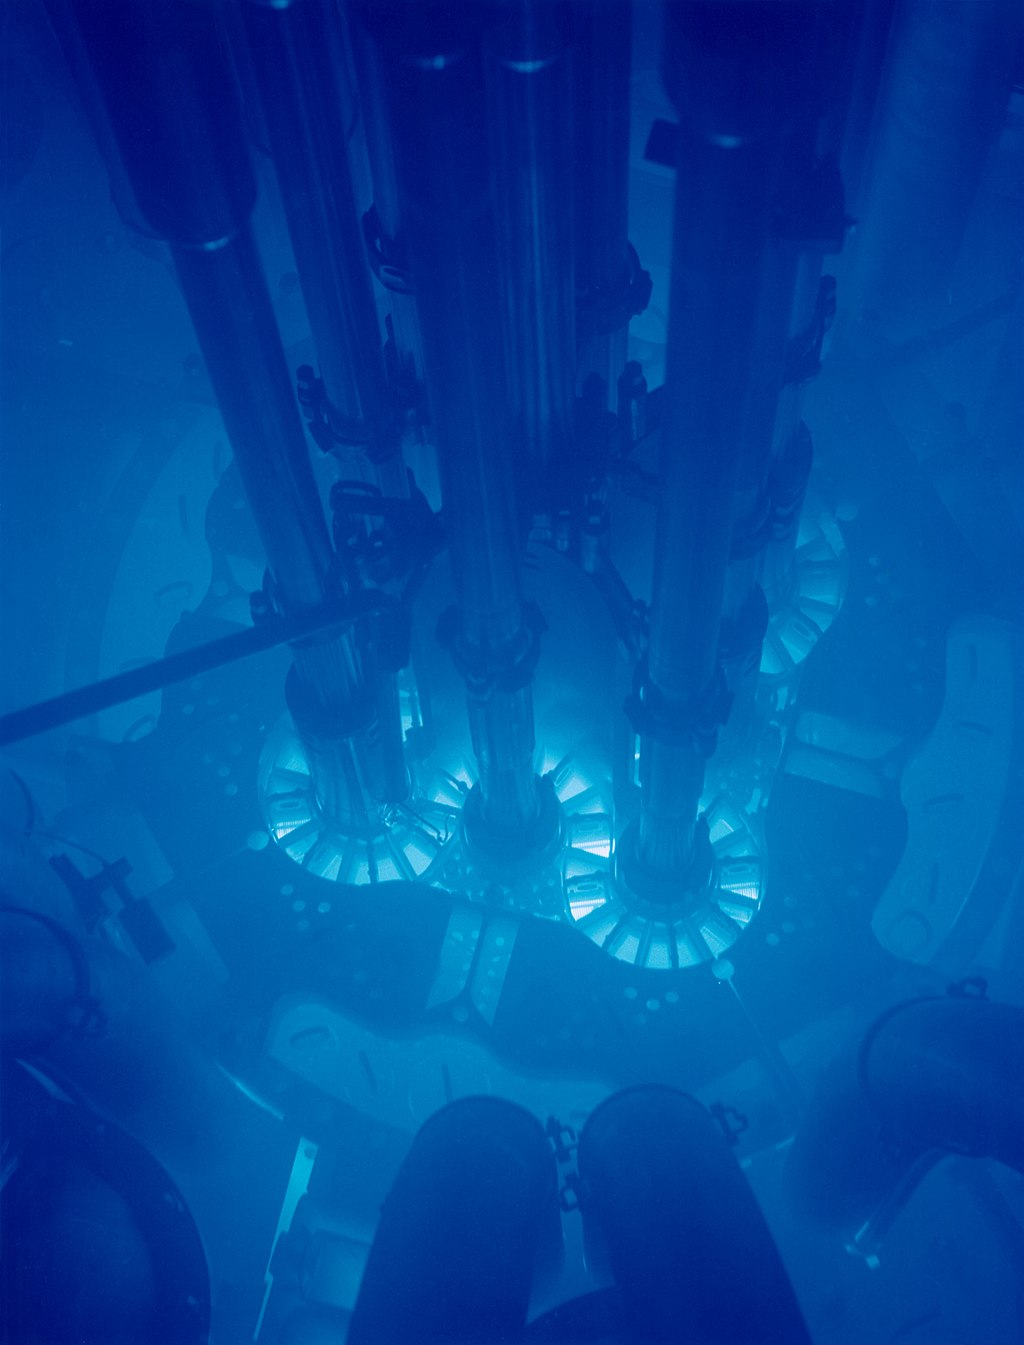
\includegraphics[height = 0.8\textwidth]{Cherenkov-reactor.jpg}
	\caption{The particles coming from the reactor core produce cherenkov radiation as they pass through the water,
	most of the produced light is "in blue"\citeFig{CherenkovReactor}}
	\label{figure: Cherenkov reactor}
\end{minipage}
\hspace{0.05\textwidth}
\begin{minipage}{0.45\textwidth}
	\centering
	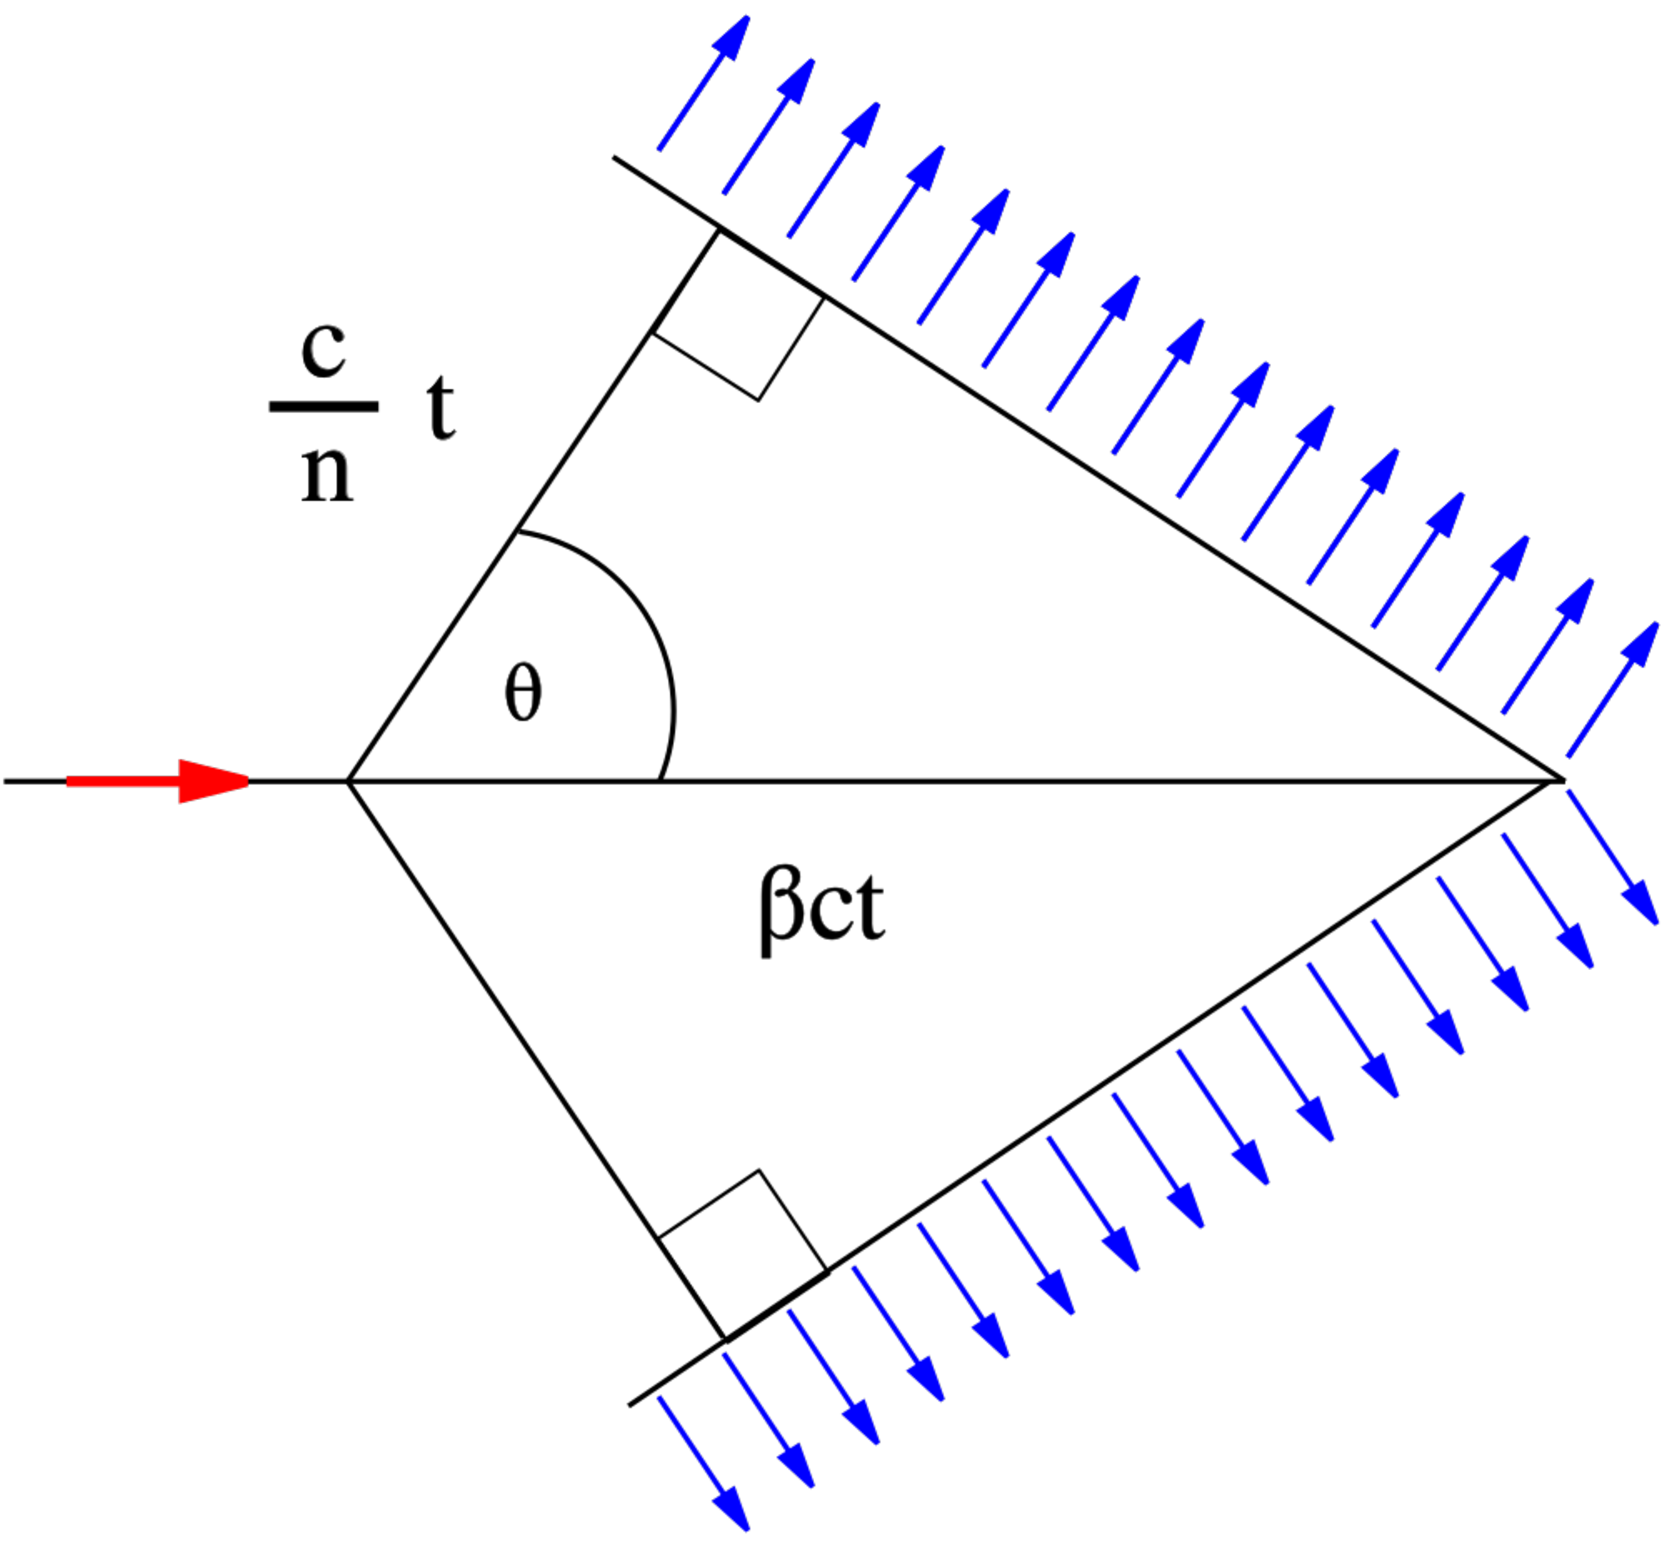
\includegraphics[height = 0.8\textwidth]{Cherenkov.pdf}
	\caption{The cone shape is reminiscent of a sonic boom, the signal is the strongest on the cone \citeFig{CherenkovIllu}}
	\label{figure: Cherenkov illustratie}
\end{minipage}
\end{figure}
Of course this is just an estimate, as the actual index of refraction is depth-dependent which
we'll get to in section \ref{section:Ice Model}.
Now this explains how the signals get generated but logically, from only knowing this
we'd expect radio waves to almost be non-existent 
due to the "in blue" nature of Cherenkov radiation. 

To understand why this isn't the case we'll need another piece of the puzzle: coherent overlap.
Coherent overlap in the radio wave spectrum range can be intuitively explained as
follows: generally the shower is of length
$\mathcal{O}$(10cm)\cite{Huege_2017}, over this length the radiation gets
emitted, most frequencies decoherently interfering, but radio waves with wavelengths of 
$\approx$ 10cm coherently interfere, and it's these waves we then wish to detect.
The radiation generated trough this Askaryan effect is called \textit{Askaryan radiation}.

The Askaryan radiation is polarized perpendicular to the Cherenkov cone, this
concept is illustrated in 2D in figure\ref{fig:illupol}.
The fact that the radiation is polarized can be useful to discern which
direction the neutrino came from using both vertically and horizontally
polarized antennae.
\begin{figure}
	\centering
	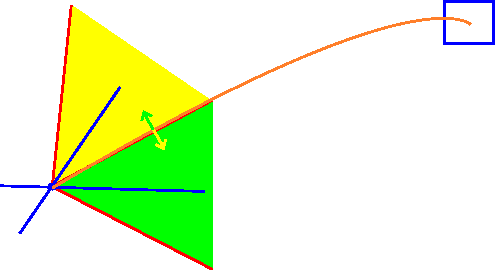
\includegraphics[width=0.5\textwidth]{illu_polarization.pdf}
	\caption{The detector receives an upwards polarization for the cherenkov cone in green
	and a downwards polarization for the one in yellow}
  	\label{fig:illupol}
\end{figure}

The radio signals that get produced by a neutrino interaction in ice always
travel along two paths, an example path is shown on figure \ref{fig:DnR}.  In
this figure the pahts are direct and refracted, designated DnR, but not that
direct and reflected (at the surface) and refracted refracted are also
possible.
\begin{figure}
  \centering
  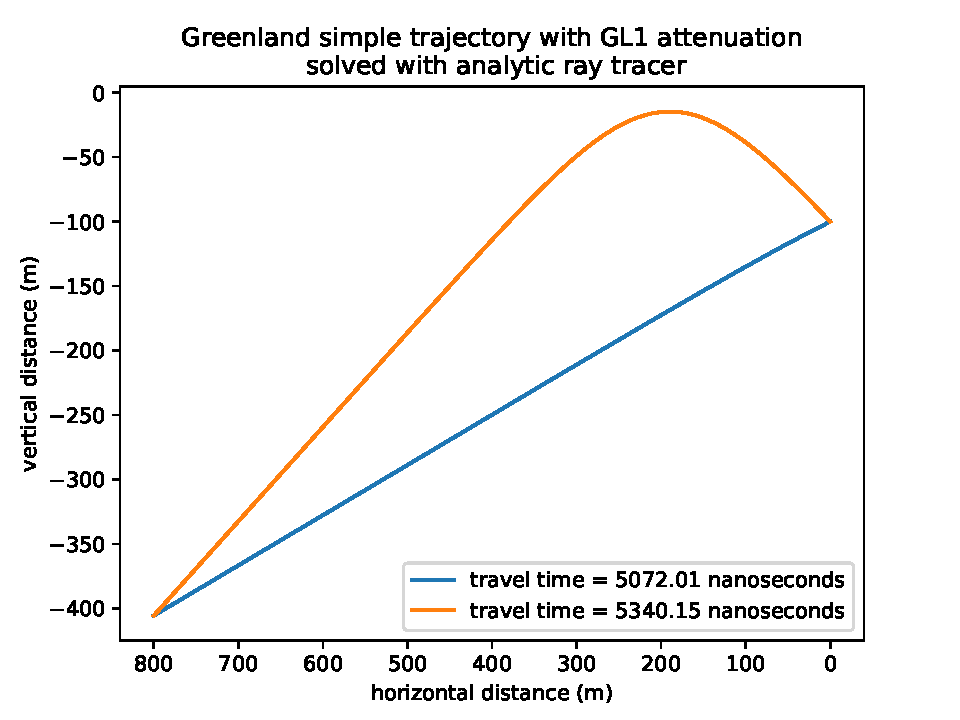
\includegraphics[width=0.7\textwidth]{DnR.pdf}
  \caption{example simulation showing both direct and refracted path from a neutrino vertex (bottom left) to a detector (top right)}
  \label{fig:DnR}
\end{figure}
This double pulse characteristic would be a smoking-gun signature of an in-ice
source.
\section{RNO-G}
Both cosmic ray and neutrino detectors face the same main problem at the
highest energies: the steeply falling flux (as was previously seen in figure
\ref{figure:Neutrino fluxes}) requires large effective areas, which leads to
the construction of neutrino detectors with volumes on the cubic kilometer
scale like IceCube\cite{IceCubeTechnical} which works on the principle of
detecting neutrinos with visible light.  But even IceCube has it's limitations,
it's still too small to observe many neutrino events above the 10 PeV
scale\cite{IceCubeGen2} in acceptable timescales. That's why a new detector was needed which was even
bigger and able to observe cosmogenic neutrinos.  We could just make IceCube
bigger but this would cost a lot of money as the individual detectors need to
be spaced closely as the attenuation length is quite short for light in the
visible spectrum propagating through ice.  

The proposed solution was to work with radio wave detectors, leveraging the
previously discussed Askaryan effect (see section \ref{sec:Askaryan}).  Radiowaves can propagate
way further in ice than visible light making it possible to space the
individual detectors further apart. The proposed location is Greenland, an
island country in North America and part of the Kingdom of Denmark which has
large ice sheets as shown in figure \ref{fig:GreenlandOP}.
\begin{figure}
  \centering
  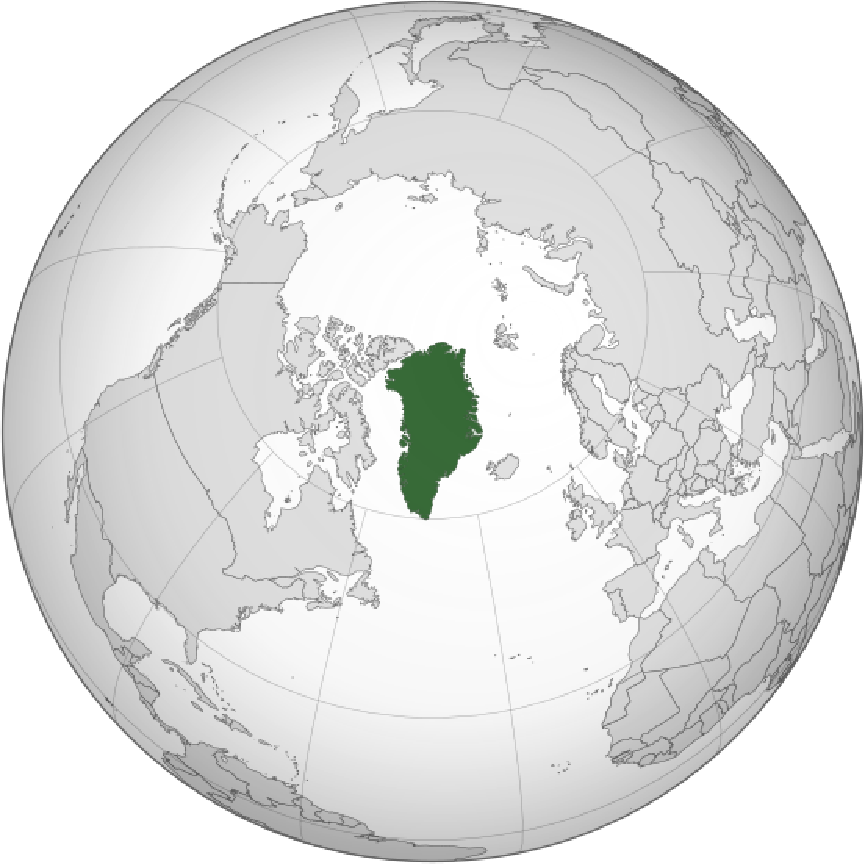
\includegraphics[width=0.5\textwidth]{figures/GreenlandOP.pdf}
  \caption{orthographic projection of Greenland with the red star representing the approximate RNO-G location\citeFig{OrthoGreenland}}
  \label{fig:GreenlandOP}
\end{figure}
The proposal for RNO-G, which was later funded and now in the construction
phase, is for it to be an array of autonomous radio stations each of which having both
surface channels and various deep channels resulting in a total of 24 channels
per station. The whole project builds heavily on the knowledge obtained through
previous radio based neutrino detectors like the NuMoon\cite{numoon} project,
ANITA\cite{ANITA}, ARA\cite{ARA},ARIANNA\cite{Barwick_2015} and RICE\cite{RICE}.
\subsection{Hardware}
A station is illustrated in figure \ref{fig:detector}, 
\begin{figure}
	\centering
	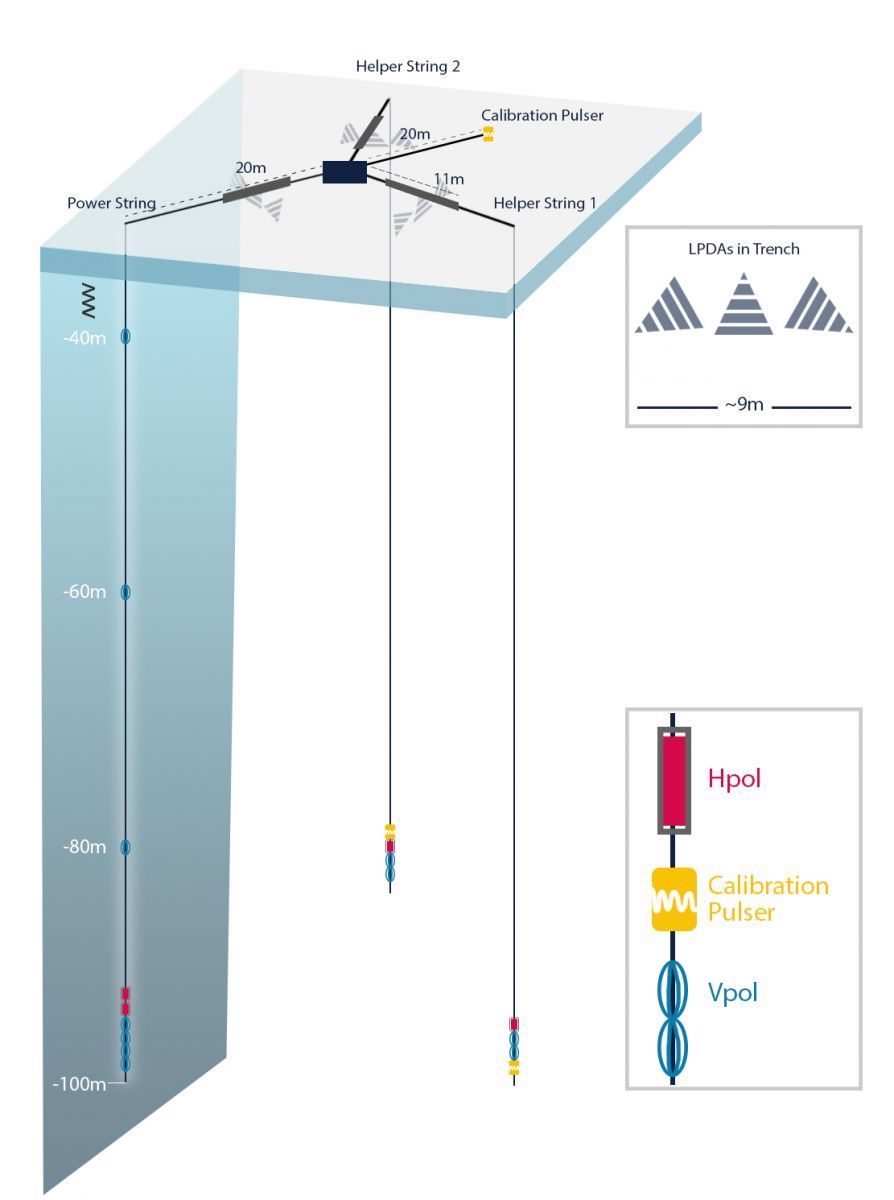
\includegraphics[height=0.4\textheight]{figures/RNO-G_station_sketch.jpg}	
	\caption{The combination of Vpol and Hpol antennae makes it possible to discern the direction of neutrinos whereas
	the surface LPDA antennae makes it possible to distinguish muons.\citeFig{DetectorIllu}}
	\label{fig:detector}
\end{figure}
the plan is to build 35 of these as is shown in figure \ref{fig:station map}. 
\begin{figure}
	\centering
	\includegraphics[width=0.55\textwidth]{figures/station-mapNoComment.png}	
	\caption{All the individual detectors are numbered but also named after various species living in
Greenland (in the native tongue)\citeFig{PlannedLay}}
	\label{fig:station map}
\end{figure}
Looking closely at one such detector we see
just below the surface 9 Log Periodic Dipole Antennas (LPDAs), these are used
to detect air shower muon signals as muons will also generate Cherenkov
radiation in the ice whose signals can then be filtered out.  Aside form these
surface detectors there are also deep components of the detector which can be
split up in three parts: Two \textit{helper strings} and the \textit{power
string}.

The helper strings are the 2 vertical cables shown on the right of figure
\ref{fig:detector} each housing 2 vertically polarized antennas (Vpols), one
quadslot antenna for the horizontal polarization component (Hpol) and one radio
pulser on each helper string which can be used to generate calibration signals.
As was previously mentioned using both the horizontal and vertical polarization of the
signal, the neutrino direction can be discerned. That's why both the helper and power 
string are equipped with both kinds of polarized antennae.

The power string (the leftmost vertical cable) is more densely instrumented
than the helper strings: At the bottom it houses a set of four Vpol and two
Hpol antennas with a spacing of 1m called the \textit{phased array}\cite{Allison_2019}. 
The phased array is an array of closely spaced antennae, due to their close spacing
their signals can be interfermetrically combined creating a coherent receiver with a 
larger aperture than the individuals. This technique is frequently used in radio astronomy
for increasing the angular resolution by combining antennae and is the main
reason it was possible to observe the black hole Sagittarius A-star\cite{SqrA*}.
It is called the "phased" array as the radio array is electronically
steered using beamformers, which is called "phasing".
The resulting high resolution arguably makes the channels in the phased array the most important 
antennae of the detector.
Then finally further up the string, with a spacing of 20m, are three more Vpol antennas.
\begin{figure}
  \centering
  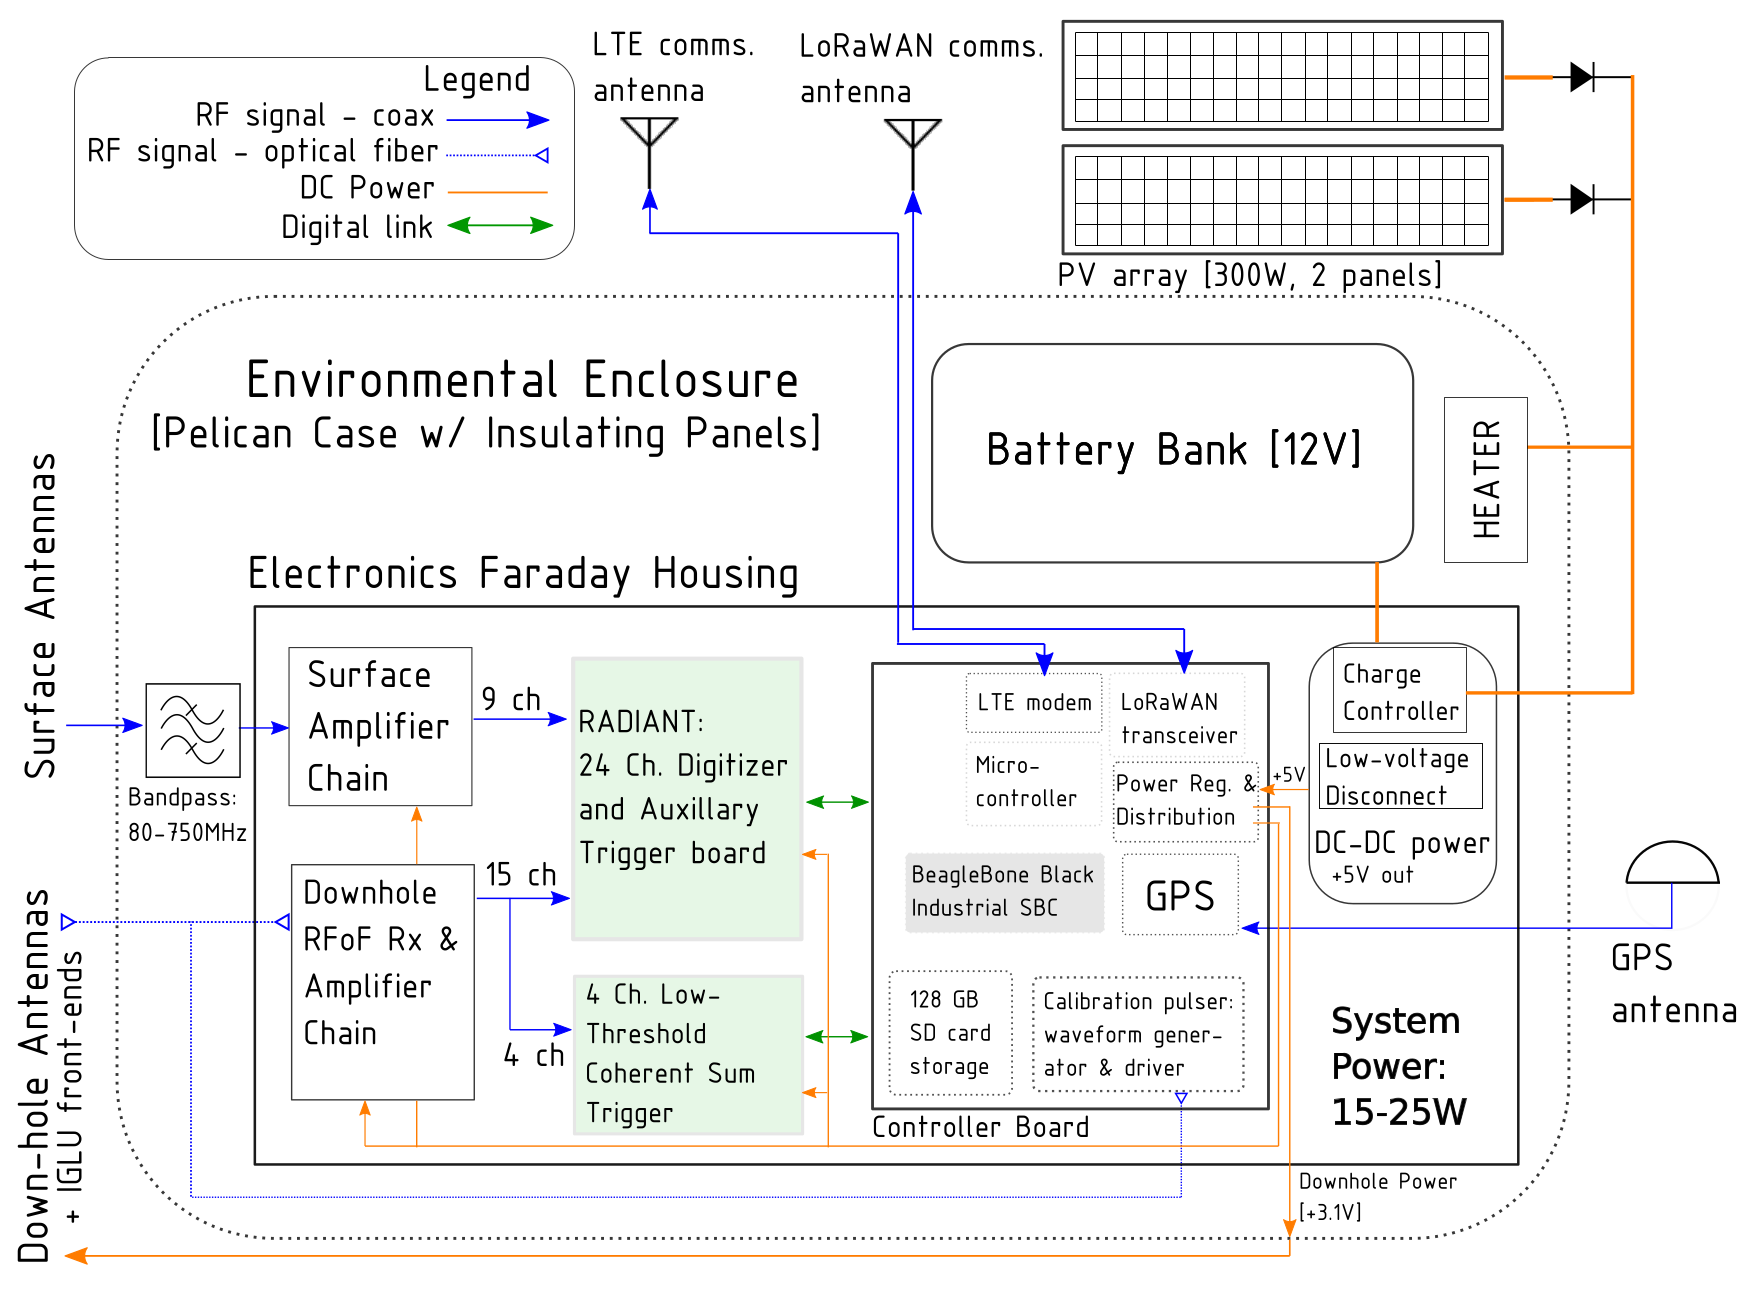
\includegraphics[width=0.85\textwidth]{SysDiagRNOG.png}
  \caption{System diagram for a RNO-G station \citeFig{Aguilar_2021_Fig}}
  \label{fig:SysDiag}
\end{figure}

A full system diagram for a RNO-G station is shown in figure \ref{fig:SysDiag},
I'll give a walk trough of how data gets collected.  The signal from each of
the deep antennae are fed into a low-noise amplifier directly above it\cite{Aguilar_2021}, from
there the signal is send to the data acquisition (DAQ) system at the surface
via a Radio Frequency over Fiber (RFoF) cable.  The signals coming from the
surface antennae are first passed through a Bandpass filter of
80-750MHz\footnote{i.e a filter that only lets frequencies in this range pass}
after which both the resulting signals and the deep component signals get sent
up to the RAdio DIgitizer and Auxiliary Neutrino Trigger (RADIANT). There it's
again amplified, digitized and, if a trigger threshold is reached, saved onto
an SD card. This data is then transmitted via a Long Term Evolution (LTE)
telecommunications network to a local server\footnote{There is additionally a
Long Range Wide Area Network (LoRaWAN) antenna as backup in case of problems
with the LTE network}, from where it is sent via a satellite link.
As a power source, battery banks are used whom are charged via solar panels.
But as there isn't enough light during the Greenland winters, there are plans to
build wind turbines (with one of the problems being the possibly detectable RF
noise the 'engine' would produce).

The two helper strings are needed for a full direction reconstruction.
Three independent measurements are needed for azimuthal information, which is
provided by the Vpol (Vertical polarization) antennas and placing the Hpol
(Horizontal polarization) antennas at different depths on every string, both
zenith and azimuth information will be provided for those signals. The helper
strings' calibration pulsers, as well as one on the surface, will ensure
regular monitoring of the performance of the station and provide information
useful for precise calibration of the antenna geometry.

\section{Reconstruction}
Now when the channels pick up a signal which has a high enough amplitude to
cause it to trigger and record the data, how would we know wether it was a neutrino
and, if so, how would we figure out it's direction?

To know wether a recorded signal was a neutrino can be quite involved but the biggest
clue is definetely the double pulse characteristic it would produce as 
a signal. Now from the recorded signal, if we know it is a neutrino,
how can we know where it came from?
We can figure this out using simulations, the code that's being used consists of 2 parts:
NuRadioMC\cite{Glaser_2020} and NuRadioReco\cite{Glaser_2019}. NuRadioMC uses
Monte Carlo simulations to generate neutrino events in the ice and simulates
how they propagate to the various channels, which will be covered more in-depth
in the next chapter. NuRadioReco is reconstruction software, it simulates how
the various detectors would respond to the detected radio waves. This simulation
software can thus be used to figure out how a signal looks like when a neutrino comes from
a certain direction and interacts at a certain point in the ice. 

A plan is to simulate a lot of neutrino events and
record the detector responses in a giant database, then, when an actual neutrino
event occurs, look in the database and match the actual
detector response to the simulated detector responses, thus finding the origin.

\section{Multi-Messenger Astronomy}
The origin of the most energetic cosmic rays is still not conclusively
identified. One approach to solving this problem is \textit{multi-messenger
astrophysics}, where several types of cosmic particles are used to identify the
sources of these ultra-high energy cosmic rays (UHECRs). E.g we simultaneously
measure gravitational waves with the Einstein telescope, neutrinos with RNO-G,
photons with various telescopes and muons with a muon detector.
